% !TeX root = tcolorbox.tex
% include file of tcolorbox.tex (manual of the LaTeX package tcolorbox)
\clearpage
\section{\mylib{external} 程序库}\label{sec:external}%
\tcbset{external/prefix=external/external_}%
通过宏包选项或在导言区中加载本程序库：
\begin{dispListing}
\tcbuselibrary{external}
\end{dispListing}

本程序库的目的是支持文档片段的外部化，例如可以独立编译的
图形或文本框。这些片段被写入外部文件，编译后将生成的
PDF 文件作为图片嵌入主文档中。
如果某个片段编译开销较大但只需编译一次或很少几次，
整个流程可以节省编译时间。

本程序库有非常好的替代方案。可以考虑使用
\refPkg{standalone} 宏包、
\refPkg{memoize} 宏包、
\refPkg{robust-externalize} 宏包，
或 \tikzname\ 外部化程序库（目前已停止维护）。
\mylib{external} 程序库介于二者之间，可以看作
\tikzname\ 外部化程序库的精简版。

\tikzname\ 外部化与 \mylib{external} 的主要区别在于：
\begin{itemize}
\item\tikzname\ |external| 以复杂方式编译整个原始文档，
  而 \mylib{external} 仅使用原始文档的导言区或其一部分。
\item\tikzname\ |external| 可以自动外部化所有 |tikzpicture| 环境，
  而 \mylib{external} 仅外部化被标记的片段。
\item 被 \mylib{external} 外部化的代码片段不限于
  |tikzpicture| 环境。但这些片段必须是独立的，
  不依赖文档的其余部分。
\end{itemize}
为什么有人会使用 \mylib{external} 而非功能更强的
\tikzname\ |external|？原因之一可能是编译速度，
但创建本程序库的主要原因是 \tikzname\ |external|
在复杂文档中容易出错——其复杂机制可能失效。
由于 \mylib{external} 不使用原始文档正文进行编译，
因此不会出现这个问题。

\begin{marker}
当源片段的 |md5| 校验和发生变化时才会重新编译。
如果仅更改了选项设置或片段外部的任何内容，
片段不会自动重新编译。
这种情况下，使用 \refKey{/tcb/external/force remake}
强制编译，或直接删除外部化的 pdf 或 md5 文件。
\end{marker}

\begin{marker}
要使用外部化选项，编译器必须带 |-shell-escape| 权限运行，
以授权可能危险的系统调用。请注意这存在安全风险。
\end{marker}


\clearpage
\subsection{为外部化准备文档}\label{subsec:external_preparation}

主文档的导言区必须包含 \refCom{tcbEXTERNALIZE} 命令。
没有此命令，不会执行任何外部化操作。

\begin{docCommand}[doc new=2015-03-11]{tcbEXTERNALIZE}{}
  在主文档导言区中使用一次此命令是外部化的必要条件。
  \emph{在此之前}的所有设置也会用于编译外部片段；
  \emph{在此之后}的所有设置在编译外部片段时将被忽略。
  如果你不确定放在哪里，将此命令放在 |\begin{document}| 正前方。

  主文档应如下所示：

\begin{dispListing}
\documentclass[a4paper]{book}%   例如
\usepackage{...}%                任意宏包
% ...
% 通常包含文档的全部或绝大部分设置。

\tcbEXTERNALIZE% 通常放在 \begin{document} 正前方

% 以下设置对独立片段完全无关紧要。
%
\begin{document}
  % 文档正文。
  % 其中也包含需要外部化的标记片段。
\end{document}
\end{dispListing}
\end{docCommand}

编译过程中，会动态创建一个 \refKey{/tcb/external/runner} 文件
（可能多次创建）。这才是编译外部化片段的实际主文件。

\begin{extTcbKey}[][doc new=2015-03-11]{runner}{=\meta{file name}}{无默认值，
  初始 \texttt{\cs{jobname}\detokenize{_run.tex}}}
设置动态创建的 |runner| 文件的 \meta{文件名}。
这是文档片段的实际主文件。
通常不需要更改初始设置。
\begin{dispListing}
\tcbset{external/runner=myrunner.tex}
\end{dispListing}
\end{extTcbKey}

\begin{extTcbKey}[][doc new=2015-03-11]{prefix}{=\meta{text}}{无默认值，
  初始 \texttt{external/}}
\meta{文本}会作为前缀添加到每个外部化片段的
\refKey{/tcb/external/name} 之前。初始设置会将所有片段
保存到 |external/| 子目录中。根据操作系统的不同，
可能需要手动创建该子目录一次。
\begin{dispListing}
% 使用"真正的"前缀而非写入子目录：
\tcbset{external/prefix=ext_}
\end{dispListing}
\end{extTcbKey}


\begin{extTcbKey}[][doc new=2015-03-11]{externalize}{\colOpt{=true\textbar false}}{默认 |true|，
  初始 |true|}
设为 |true| 时，标记的片段在需要时编译。
设为 |false| 时，标记的片段不编译，而是作为文本包含。
\refKey{/tcb/external/externalize} 只能在 \refCom{tcbEXTERNALIZE} 之后使用。
\end{extTcbKey}

\begin{extTcbKey}[][doc new=2015-03-11]{force remake}{\colOpt{=true\textbar false}}{默认 |true|，
  初始 |false|}
设为 |true| 时，标记的片段始终编译。
设为 |false| 时，标记的片段仅在需要时编译。
当缺少已编译的 pdf 文件或源片段的 |md5| 校验和发生变化时，即为需要编译。
\end{extTcbKey}

\enlargethispage*{1cm}
\begin{extTcbKey}[][doc new and updated={2015-03-11}{2017-02-24}]{\tcbexclamation}{}{style}
  将 \refKey{/tcb/external/force remake} 设为 |true| 的快捷方式。
\end{extTcbKey}

\begin{extTcbKey}[][doc new and updated={2015-06-12}{2017-02-24}]{-}{}{style}
  将 \refKey{/tcb/external/externalize} 设为 |false| 的快捷方式。
\end{extTcbKey}


\subsection{标记外部化片段}\label{subsec:external_marking}

\begin{docEnvironment}[doc new=2015-03-11]{tcbexternal}{\oarg{options}\marg{name}}
将环境内容标记为待外部化的片段。
通常内容是 |tikzpicture| 或类似图形。
请注意，片段不应与文档其余部分有任何依赖关系，
例如不能引用计数器或设置计数器。
\meta{名称}会自动添加 \refKey{/tcb/external/prefix} 前缀。
组合起来必须是唯一的文件名。建议名称中不使用空格或变音符号。
\meta{选项}取自 |/tcb/external/| 键树。

\begin{dispExample}
\begin{tcbexternal}{example_tikzpicture}
  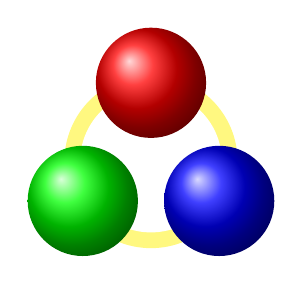
\begin{tikzpicture}
    \path[fill=yellow!50!white] (0,0) circle (11mm);
    \path[fill=white] (0,0) circle (9mm);
    \foreach \w/\c in {90/red,210/green,330/blue}
      {\path[shading=ball,ball color=\c] (\w:1cm) circle (7mm);}
  \end{tikzpicture}
\end{tcbexternal}
\end{dispExample}

\medskip

如果要外部化 \refEnv{tcolorbox}，应对文本框使用
\refKey{/tcb/nobeforeafter}。与前后文本的缩进和间距
必须在 \refEnv{tcbexternal} 环境之外单独设置。

\begin{dispExample}
\noindent%
\begin{tcbexternal}[minipage]{example_tcolorbox}
  \begin{tcolorbox}[nobeforeafter,enhanced,
      fonttitle=\bfseries,title=外部化文本框,
      colframe=red!50!black,drop fuzzy shadow,
      interior style={fill overzoom image=goldshade.png}]
    这个完整的 tcolorbox 被外部化了。此处不能使用编号文本框。
    注意 \texttt{minipage} 选项，它将当前行宽告知外部片段。
  \end{tcolorbox}
\end{tcbexternal}
\end{dispExample}

\begin{dispExample}
\begin{tcolorbox}[nobeforeafter,enhanced,
      fonttitle=\bfseries,title=外部化文本框,
      colframe=blue!50!black,
      interior style={fill overzoom image=blueshade.png}]
  \begin{tcbexternal}[minipage]{example_tcolorbox2}
    \color{white}%
    该 tcolorbox 的内部内容被外部化了。
    可以毫无问题地使用编号文本框。
    注意文本颜色需要手动设置，因为它被转换为图片。
  \end{tcbexternal}
\end{tcolorbox}
\end{dispExample}

\begin{dispExample}
\begin{tcbexternal}[minipage]{example_tabularx}
  \newcolumntype{Y}{>{\raggedleft\arraybackslash}X}%
  \begin{tabularx}{\linewidth}{|l||Y|Y|Y|Y||Y|}\hline
    组 & 一 & 二 & 三 & 四 & 合计\\\hline\hline
    红 & 1000.00 & 2000.00 & 3000.00 & 4000.00 & 10000.00\\\hline
    绿 & 2000.00 & 3000.00 & 4000.00 & 5000.00 & 14000.00\\\hline
    蓝 & 3000.00 & 4000.00 & 5000.00 & 6000.00 & 18000.00\\\hline\hline
    合计 & 6000.00 & 9000.00 & 12000.00 & 15000.00 & 42000.00\\\hline
  \end{tabularx}
\end{tcbexternal}
\end{dispExample}


\end{docEnvironment}

\begin{extTcbKey}[][doc new=2015-03-11]{name}{=\meta{name}}{无默认值，
  初始 \texttt{unnamed}}
\meta{名称}会自动添加 \refKey{/tcb/external/prefix} 前缀。
组合起来必须是外部化的唯一文件名。
通常不直接使用此键，而是作为必填参数间接设置，
参见 \refEnv{tcbexternal}。
\end{extTcbKey}


\clearpage
\begin{docEnvironment}[doc new=2015-03-11]{extcolorbox}{\oarg{options}\marg{name}\oarg{tcolorbox options}}
  这是 \refEnv{tcolorbox} 的外部化版本，通过
  \refCom{newtcbexternalizetcolorbox} 创建：
\begin{dispListing}
\newtcbexternalizetcolorbox{extcolorbox}{tcolorbox}{}{}
\end{dispListing}
  \meta{选项}和 \meta{名称}传递给底层的 \refEnv{tcbexternal} 环境，
  而 \meta{tcolorbox 选项}传递给 \refEnv{tcolorbox}。

  \begin{marker}
  请注意，不应在 \meta{tcolorbox 选项}中重新定义
  \refKey{/tcb/before} 和 \refKey{/tcb/after}，
  否则外部化版本与非外部化版本将不一致。
  \end{marker}

\begin{dispExample}
\begin{extcolorbox}[minipage]{example_extcolorbox}
  [ enhanced,colframe=red!50!black,colback=yellow!10,
    fonttitle=\bfseries,drop fuzzy shadow,
    title=我的外部框 ]

  此文本框已完全外部化。

  \begin{tcolorbox}[colframe=blue,colback=blue!5,before skip=6pt]
  内部框。
  \end{tcolorbox}
\end{extcolorbox}
\end{dispExample}
\end{docEnvironment}

\begin{marker}
\begin{itemize}
\item\textbf{切勿}外部化编号文本框。
\item\textbf{切勿}外部化包含对其他内容引用的文本框，
  例如使用 |\ref| 或 |\cite|。
\item\textbf{切勿}外部化可跨页断开的文本框。
\end{itemize}
\kern6pt
\end{marker}

\clearpage
\begin{docEnvironment}[doc new=2015-03-11]{extikzpicture}{\oarg{options}\marg{name}\oarg{tikz options}}
  这是 |tikzpicture| 的外部化版本，通过
  \refCom{newtcbexternalizeenvironment} 创建：
\begin{dispListing}
\newtcbexternalizeenvironment{extikzpicture}{tikzpicture}{}{}{}
\end{dispListing}
  \meta{选项}和 \meta{名称}传递给底层的 \refEnv{tcbexternal} 环境，
  而 \meta{tikz 选项}传递给 |tikzpicture|。

\tcbset{/tcb/external/externalize}%----- 即使全局关闭也执行外部化
\begin{dispExample}
\begin{center}
\begin{extikzpicture}[
  preamble={\usepackage{pgfplots}},  % 为外部图形添加宏包
  input source on error=false,       % 出错时不加载源码
]{example_pgfplots}
  \pgfplotsset{width=12cm}
  \begin{axis}[3d box=background,grid=major,
    xlabel=$x$, ylabel=$y$, zlabel=$z$, view/h=40,
    mesh/interior colormap name=hot,
    colormap/blackwhite,
    z buffer=sort,domain=0:90,y domain=0:60,
    zmin=0,zmax=2,z post scale=1.2,
    ]
  \addplot3[surf,mesh/interior colormap name=blackwhite,
    colormap/hot,] ( {cos(x)},{sin(x)}, {2*sin(y)} );
  \addplot3[surf] ( {2*cos(x)*cos(y)},{2*sin(x)*cos(y)}, {2*sin(y)} );
  \end{axis}
\end{extikzpicture}
\end{center}
\end{dispExample}

\end{docEnvironment}




\clearpage
\begin{docTcbKey}[][doc new=2015-03-11]{externalize listing}{=\meta{name}}{样式，无默认值}
  将 \refEnv{tcblisting} 的文本内容以给定的 \meta{名称}外部化。
  注意代码列表部分不会被外部化。
\end{docTcbKey}


\begin{dispExample}
\begin{tcblisting}{externalize listing=example_listing,
  bicolor,colback=yellow!10,colframe=yellow!50!black,
  colbacklower=white,center lower}
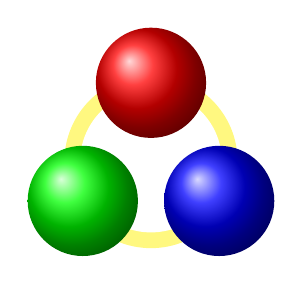
\begin{tikzpicture}
  \path[fill=yellow!50!white] (0,0) circle (11mm);
  \path[fill=white] (0,0) circle (9mm);
  \foreach \w/\c in {90/red,210/green,330/blue}
    {\path[shading=ball,ball color=\c] (\w:1cm) circle (7mm);}
\end{tikzpicture}
\end{tcblisting}
\end{dispExample}


\begin{docTcbKey}[][doc new=2015-03-11]{externalize listing\tcbexclamation}{=\meta{name}}{样式，无默认值}
\refKey{/tcb/externalize listing} 与 \refKey{/tcb/external/force remake} 的组合。
\end{docTcbKey}

\begin{docTcbKey}[][doc new=2015-03-11]{externalize example}{=\meta{name}}{样式，无默认值}
  将 \refEnv{dispExample*} 的文本内容以给定的 \meta{名称}外部化。
  注意代码列表部分不会被外部化。

\begin{dispExample}
\begin{dispExample*}{sidebyside,externalize example=example_example}
\tikz\path[shading=ball,
  ball color=red] circle (7mm);
\end{dispExample*}
\end{dispExample}
\end{docTcbKey}

\begin{docTcbKey}[][doc new=2015-03-11]{externalize example\tcbexclamation}{=\meta{name}}{样式，无默认值}
\refKey{/tcb/externalize example} 与 \refKey{/tcb/external/force remake} 的组合。
\end{docTcbKey}

\clearpage
\subsection{自定义设置}\label{subsec:external_custom}

\begin{extTcbKey}[][doc new=2015-03-11]{safety}{=\meta{length}}{无默认值，
  初始 |2mm|}
片段框外围环绕一个厚度为 \meta{长度} 的安全边距。
该边距在图片插入时自动裁剪。
此机制的目的是捕获超出边界框的框内容。
例如，|tcolorbox| 的阴影绘制在边界框之外，
否则会被裁掉。
\end{extTcbKey}

\begin{extTcbKey}[][doc new=2015-03-11]{environment}{=\meta{env}}{无默认值，初始未设置}
用不带参数的环境 \meta{env} 包裹导出的片段文本。
注意，此选项对 \refKey{/tcb/externalize listing} 无效。
\end{extTcbKey}

\begin{extTcbKey}[][doc new=2015-05-05]{environment with percent}{\colOpt{=true\textbar false}}{默认 |true|，
  初始 |true|}
设为 |true| 时，\refKey{/tcb/external/environment} 的
|\begin| 和 |\end| 代码后追加百分号。对于逐字环境，
此选项通常需设为 |false|。
\end{extTcbKey}


\begin{extTcbKey}[][doc new=2015-03-11]{minipage}{\colOpt{=\meta{length}}}{默认 \texttt{\cs{linewidth}}，
  初始未设置}
用 minipage 包裹导出的片段文本。可选的 \meta{长度}
参数设置 minipage 的宽度。注意默认宽度是主文档的当前行宽。
示例参见 \refEnv{tcbexternal}。
注意，此选项对 \refKey{/tcb/externalize listing} 无效。
\end{extTcbKey}


\begin{extTcbKey}[][doc new=2015-03-11]{plain}{}{无取值，初始已设置}
移除所有为包裹片段而设置的文本。
这会移除 \refKey{/tcb/external/minipage} 的设置，
但与 \refKey{/tcb/external/safety} 无关。
\end{extTcbKey}


\begin{extTcbKey}[][doc new=2015-03-11]{compiler}{=\meta{text}}{无默认值，
  初始 \texttt{pdflatex}}
设置编译片段的编译器名称。
\end{extTcbKey}

\begin{extTcbKey}[][doc new=2015-03-11]{runs}{=\meta{number}}{无默认值，
  初始 |1|}
设置片段的编译次数。
\begin{dispExample}
\begin{tcbexternal}[minipage,runs=2]{example_raster}
  \begin{tcbitemize}[raster equal height,
      size=small,colframe=red!50!black,colback=red!10!white]
    \tcbitem 一
    \tcbitem \Huge 二
    \tcbitem 三
    \tcbitem 四
  \end{tcbitemize}
\end{tcbexternal}
\end{dispExample}
\end{extTcbKey}

\enlargethispage*{1cm}
\begin{extTcbKey}[][doc new=2015-03-11]{input source on error}{\colOpt{=true\textbar false}}{默认 |true|，
  初始 |true|}
设为 |true| 时，加载片段源代码而非失败的 pdf 图片。
通常这会在源代码出错处停止，有助于检测原因。
如果源码输入编译无误，则文档设置可能不正确，
参见 \zvref{subsec:external_preparation}。
这种情况下可能需要手动创建 |external/| 子目录，
参见 \refKey{/tcb/external/prefix}。\par
如果选项设为 |false|，编译遇到错误立即停止。
此时需查阅外部片段的日志文件以获取错误信息。
\end{extTcbKey}


\clearpage

\begin{extTcbKey}[][doc new=2015-05-05]{preclass}{=\meta{code}}{无默认值，
  初始未设置}
给定的 \meta{代码}添加到片段文档之前。
通常这意味着在 |\documentclass| 之前。
不用于主文档的编译。
\end{extTcbKey}


\begin{extTcbKey}[][doc new=2015-05-05]{PassOptionsToPackage}{=\marg{options}\marg{package}}{无默认值，
  初始未设置}
将给定的 \meta{选项}传递给片段文档的指定 \meta{宏包}。
这是使用 \refKey{/tcb/external/preclass} 配合
|\PassOptionsToPackage| 的快捷方式。
不用于主文档的编译。
\end{extTcbKey}


\begin{extTcbKey}[][doc new=2015-05-05]{PassOptionsToClass}{=\marg{options}\marg{class}}{无默认值，
  初始未设置}
将给定的 \meta{选项}传递给片段文档的指定 \meta{文档类}。
这是使用 \refKey{/tcb/external/preclass} 配合
|\PassOptionsToClass| 的快捷方式。
不用于主文档的编译。
\end{extTcbKey}


\begin{extTcbKey}[][doc new=2015-05-05]{clear preclass}{}{无取值}
移除所有额外的 \refKey{/tcb/external/preclass} 设置。
\end{extTcbKey}



\begin{extTcbKey}[][doc new=2015-03-11]{preamble}{=\meta{code}}{无默认值，
  初始未设置}
给定的 \meta{代码}添加到片段文档的导言区。
不用于主文档的编译。
\end{extTcbKey}


\begin{extTcbKey}[][doc new=2015-05-05]{preamble tcbset}{=\meta{options}}{无默认值，
  初始未设置}
将给定的 \meta{选项}作为 \refCom{tcbset} 的参数
添加到片段文档的导言区。
不用于主文档的编译。
\end{extTcbKey}


\begin{extTcbKey}[][doc new=2015-03-16]{clear preamble}{}{无取值}
移除所有额外的 \refKey{/tcb/external/preamble} 设置。
\end{extTcbKey}



\begin{docCommand}[doc new=2015-03-11]{tcbifexternal}{\marg{true}\marg{false}}
  在片段编译时展开为 \meta{true}，
  在主文档编译时展开为 \meta{false}。
 可在 \refCom{tcbEXTERNALIZE} \emph{之前}使用此命令，
  为片段和主文档提供不同的设置。
\begin{dispListing}
\tcbifexternal{
  \usepackage{onlyforexternal}
}{
  \usepackage{onlyformain}
}
\end{dispListing}
\end{docCommand}



\clearpage
\begin{docCommand}[doc new=2015-03-11]{newtcbexternalizeenvironment}{\marg{newenv}\marg{env}\marg{options}\marg{begin}\marg{end}}
  创建一个基于 \refEnv{tcbexternal} 的新环境 \meta{newenv}。
  此环境\emph{至少}接受一个可选参数和一个必填参数。
  这两个参数传递给 \refEnv{tcbexternal}。
  此外，给定的 \meta{选项}始终添加到 \refEnv{tcbexternal} 的选项列表中。\par
  环境内容被外部化，外部片段由环境 \meta{env} 包裹。
  \meta{newenv} 的所有后续参数作为参数传递给 \meta{env}。\par
  嵌入的图片前添加 \meta{begin}，后添加 \meta{end}。\par
  \refEnv{extikzpicture} 是 \refCom{newtcbexternalizeenvironment} 的应用示例。

\begin{dispExample}
\newtcbexternalizeenvironment{extabular}{tabular}{}{\par\centering}{\par}

\begin{extabular}{example_tabular}{|l|p{6cm}|r|}\hline
A & B & C\\\hline
a & 此表格作为片段外部化。显然，
  这仅对高度复杂的表格才有意义。
& b\\\hline
\end{extabular}
\end{dispExample}
\end{docCommand}


\begin{docCommand}[doc new=2015-03-11]{renewtcbexternalizeenvironment}{\marg{newenv}\marg{env}\marg{options}\marg{begin}\marg{end}}
  与 \refCom{newtcbexternalizeenvironment} 相同，但环境 \meta{newenv}
  由 |\renewenvironment| 而非 |\newenvironment| 创建。
\end{docCommand}


\begin{docCommand}[doc new=2015-03-11]{newtcbexternalizetcolorbox}{\marg{newenv}\marg{env}\marg{options}\marg{begin end options}}
  创建一个基于 \refEnv{tcbexternal} 的新环境 \meta{newenv}。
  此环境\emph{至少}接受一个可选参数和一个必填参数。
  这两个参数传递给 \refEnv{tcbexternal}。
  此外，给定的 \meta{选项}始终添加到 \refEnv{tcbexternal} 的选项列表中。\par
  环境内容被外部化，外部片段由环境 \meta{env} 包裹。
  \meta{newenv} 的所有后续参数作为参数传递给 \meta{env}。
  \textbf{与 \refCom{newtcbexternalizeenvironment} 不同的是，
  环境 \meta{env}应基于 \refEnv{tcolorbox} 或 \refEnv{tcblisting}。}\par
  \meta{begin end 选项}是用于设置嵌入图片前后间距的选项，
  使用 \refKey{/tcb/before}、\refKey{/tcb/before skip}、
  \refKey{/tcb/after} 或 \refKey{/tcb/after skip}。
  \begin{marker}
  在 \meta{begin end 选项}中使用与定义 \meta{env} 时
  \refKey{/tcb/before} 和 \refKey{/tcb/after} 完全相同的值！
  否则外部化版本与非外部化版本的间距将不同。
  \end{marker}
  \refEnv{extcolorbox} 是 \refCom{newtcbexternalizetcolorbox} 的应用示例。


\inputpreamblelisting{M}

{
\tcbset{external/preamble={\input{tcolorbox_preamble_M.tex}}}
\begin{dispExample}
\begin{exmyownlisting}{example_mylisting}% <- 外部文件名
  {我的外部化示例框}
这是我的 \LaTeX\ 框。
\end{exmyownlisting}
\end{dispExample}
}
\end{docCommand}


\begin{docCommand}[doc new=2015-03-11]{renewtcbexternalizetcolorbox}{\marg{newenv}\marg{env}\marg{options}\marg{begin end options}}
  与 \refCom{newtcbexternalizetcolorbox} 相同，但环境 \meta{newenv}
  由 |\renewenvironment| 而非 |\newenvironment| 创建。
\end{docCommand}


\begin{docCommand}[doc new=2016-07-14]{tcbiffileprocess}{\marg{condition}\marg{source}\marg{md5-file}\marg{target}\marg{true}\marg{false}}
  这是内部使用的底层宏。
 将 \meta{源}文件的 MD5 摘要与辅助 \meta{md5 文件}中
  存储的 MD5 摘要进行比较。
  如果二者不同，更新辅助 \meta{md5 文件}以存储当前 MD5 摘要。此外，
  \begin{itemize}
  \item 如果 \meta{条件}等于 |0|，执行 \meta{true}。
  \item 如果 \meta{条件}等于 |1|：\\
    如果当前与存储的 MD5 摘要不同，执行 \meta{true}。\\
    否则，如果 \meta{目标}文件不存在，执行 \meta{true}。\\
    否则，如果 \meta{目标}文件比 \meta{md5 文件}旧，执行 \meta{true}。\\
    否则，执行 \meta{false}。
  \item 如果 \meta{条件}等于 |2|，执行 \meta{false}。
  \end{itemize}
  \meta{true}代码的预期处理目的是从给定的 \meta{源}文件
  生成 \meta{目标}文件。
\end{docCommand}


\clearpage
\subsection{故障排除与常见问题}\label{subsec:external_troubleshooting}

\begin{itemize}

\item\textbf{我使用默认设置，但 |external| 子目录没有被创建。}\\
  根据操作系统和编译器的不同，|external| 子目录可能自动创建或不创建。
  如果没有，请手动创建该目录，或在文档中添加以下内容：
\begin{dispListing}
\ExplSyntaxOn
\sys_shell_now:n { mkdir~external }
\ExplSyntaxOff
\end{dispListing}
或
\begin{dispListing}
\ExplSyntaxOn
\sys_shell_now:n { mkdir~-p~external }
\ExplSyntaxOff
\end{dispListing}
  如果 \refKey{/tcb/external/prefix} 与所选片段名称的组合
  指向 |external| 之外的其他子目录，则需要相应调整。

\item\textbf{我使用 \refPkg{minted} 宏包，每个外部化片段都会生成一个缓存目录。}\\
  要避免此问题，有多种方法。
  \begin{itemize}
  \item 如果片段代码中不需要 |minted|，可以在 \refCom{tcbEXTERNALIZE}
    \emph{之后}使用 |\usepackage{minted}|，
    或使用 \refCom{tcbifexternal} 为外部代码关闭 |minted|。
    如果 \refPkg{minted} 已被其他宏包加载，在导言区添加：
\begin{dispListing}
\tcbset{external/PassOptionsToPackage={draft}{minted}}
\end{dispListing}
  \item 如果片段代码需要 |minted|，可以在导言区添加以下内容关闭缓存：
\begin{dispListing}
\tcbset{external/PassOptionsToPackage={cache=false}{minted}}
\end{dispListing}
  或者，可以使用 |minted| 的 |cachedir| 选项重定向缓存。
  \end{itemize}


\end{itemize}

